\documentclass[12pt, a4paper]{article}

\usepackage[T2A]{fontenc}
\usepackage[utf8]{inputenc}
\usepackage[main=russian, english]{babel}

\usepackage{microtype}
\sloppy


%% ГОСТ 7.32-2017
%% 6.1 Общие требования
%%
%% 6.1.1 Изложение текста и оформление отчёта выполняют в соответствии с требованиями настоящего стандарта.
%% Страницы текста отчёта о НИР и включённые в отчёт иллюстрации и таблицы должны соответствовать формату А4 по ГОСТ 9327.
%% Допускается применение формата А3 при наличии большого количества таблиц и иллюстраций данного формата.
%%
%% Отчёт о НИР должен быть выполнен любым печатным способом на одной стороне листа белой бумаги формата А4 через полтора интервала.

\usepackage[onehalfspacing]{setspace}

%% Допускается при подготовке заключительного отчёта о НИР печатать через один интервал, если отчёт имеет значительный объём (500 и более страниц).
%% Цвет шрифта должен быть чёрным, размер шрифта — не менее 12 пт.
%% Рекомендуемый тип шрифта для основного текста отчёта — Times New Roman.

%\usepackage{paratype}
%\renewcommand{\rmdefault}{PTSerif-TLF}
%\renewcommand{\ttdefault}{PTMono-TLF}

%% Полужирный шрифт применяют только для заголовков разделов и подразделов, заголовков структурных элементов.
%% Использование курсива допускается для обозначения объектов (биология, геология, медицина, нанотехнологии, генная инженерия и др.) и написания терминов (например, in vivo, in vitro) и иных объектов и терминов на латыни.
%%
%% Для акцентирования внимания может применяться выделение текста с помощью шрифта иного начертания, чем шрифт основного текста, но того же кегля и гарнитуры.
%% Разрешается для написания определённых терминов, формул, теорем применять шрифты разной гарнитуры.
%%
%% Текст отчёта следует печатать, соблюдая следующие размеры полей: левое — 30 мм, правое — 15 мм, верхнее и нижнее — 20 мм.

\newcommand{\PageLeftMargin}{30mm}
\newcommand{\PageRightMargin}{15mm}
\newcommand{\PageTopMargin}{20mm}
\newcommand{\PageBottomMargin}{20mm}

\usepackage[
	left=\PageLeftMargin,
	right=\PageRightMargin,
	top=\PageTopMargin,
	bottom=\PageBottomMargin,
]{geometry}

%% Абзацный отступ должен быть одинаковым по всему тексту отчёта и равен 1,25 см.

\usepackage{indentfirst}
\setlength{\parindent}{1.25cm}

\setlength{\parskip}{1ex}

%%
%% 6.1.2 Вне зависимости от способа выполнения отчёта качество напечатанного текста и оформления иллюстраций, таблиц, распечаток программ должно удовлетворять требованию их чёткого воспроизведения.
%%
%% 6.1.3 При выполнении отчёта о НИР необходимо соблюдать равномерную плотность и чёткость изображения по всему отчёту.
%% Все линии, буквы, цифры и знаки должны иметь одинаковую контрастность по всему тексту отчёта.
%%
%% 6.1.4 Фамилии, наименования учреждений, организаций, фирм, наименования изделий и другие имена собственные в отчёте приводят на языке оригинала.
%% Допускается транслитерировать имена собственные и приводить наименования организаций в переводе на язык отчёта с добавлением (при первом упоминании) оригинального названия по ГОСТ 7.79.
%%
%% 6.1.5 Сокращения слов и словосочетаний на русском, белорусском [1] и иностранных европейских языках оформляют в соответствии с требованиями ГОСТ 7.11, ГОСТ 7.12.
%%   [1] Для Республики Беларусь применим СТБ 7.12.
%%
%% 6.2 Построение отчёта
%%
%% 6.2.1 Наименования структурных элементов отчёта: "СПИСОК ИСПОЛНИТЕЛЕЙ", "РЕФЕРАТ", "СОДЕРЖАНИЕ", "ТЕРМИНЫ И ОПРЕДЕЛЕНИЯ", "ПЕРЕЧЕНЬ СОКРАЩЕНИЙ И ОБОЗНАЧЕНИЙ", "ВВЕДЕНИЕ", "ЗАКЛЮЧЕНИЕ", "СПИСОК ИСПОЛЬЗОВАННЫХ ИСТОЧНИКОВ", "ПРИЛОЖЕНИЕ" служат заголовками структурных элементов отчёта.

\AtBeginDocument{\renewcommand\contentsname{Содержание}}

%%
%% Заголовки структурных элементов следует располагать в середине строки без точки в конце, прописными буквами, не подчёркивая.
%% Каждый структурный элемент и каждый раздел основной части отчёта начинают с новой страницы.

\usepackage{titlesec}

\newcommand{\ChapterLeftMargin}{}
\newcommand{\ChapterFormat}{}
\newcommand{\ChapterSep}{}
\newcommand{\ChapterBeforeCode}{}

\newcommand{\SetMainPartChapterSettings}{%
	\renewcommand{\ChapterLeftMargin}{\parindent}%
	\renewcommand{\ChapterFormat}{\bfseries}%
	\renewcommand{\ChapterSep}{1em}%
	\renewcommand{\ChapterBeforeCode}{}%
}

\newcommand{\SetStructuralElementChapterSettings}{%
	\renewcommand{\ChapterLeftMargin}{0pt}%
	\renewcommand{\ChapterFormat}{\filcenter\bfseries}%
	\renewcommand{\ChapterSep}{}%
	\renewcommand{\ChapterBeforeCode}{\MakeUppercase}%
}

\SetStructuralElementChapterSettings

\titlespacing*{\chapter}{\ChapterLeftMargin}{-30pt}{8pt}
\titleformat{\chapter}[block]{\ChapterFormat}{\thechapter}{\ChapterSep}{\ChapterBeforeCode}{}

\newcommand{\StructuralElement}[1]{%
	\chapter*{#1}%
	\addcontentsline{toc}{chapter}{\MakeUppercase{#1}}%
}

\newenvironment{MainPart}%
	{\SetMainPartChapterSettings}%
	{\SetStructuralElementChapterSettings}

%%
%% 6.2.2 Основную часть отчёта следует делить на разделы, подразделы и пункты.
%% Пункты при необходимости могут делиться на подпункты.
%% Разделы и подразделы отчёта должны иметь заголовки.
%% Пункты и подпункты, как правило, заголовков не имеют.
%%
%% 6.2.3 Заголовки разделов и подразделов основной части отчёта следует начинать с абзацного отступа и размещать после порядкового номера, печатать с прописной буквы, полужирным шрифтом, не подчёркивать, без точки в конце.
%% Пункты и подпункты могут иметь только порядковый номер без заголовка, начинающийся с абзацного отступа.

\titlespacing*{\section}{\parindent}{*4}{*2}
\titlespacing*{\subsection}{\parindent}{*4}{*4}
\titlespacing*{\subsubsection}{\parindent}{*4}{*4}
\titlespacing*{\paragraph}{\parindent}{*0}{*1}
\titleformat{\section}{\bfseries}{\thesection}{1em}{}{}{}
\titleformat{\subsection}{\bfseries}{\thesubsection}{1em}{}{}{}
\titleformat{\subsubsection}{\bfseries}{\thesubsubsection}{1em}{}{}{}

%%
%% 6.2.4 Если заголовок включает несколько предложений, их разделяют точками.
%% Переносы слов в заголовках не допускаются.
%%
%% 6.3 Нумерация страниц отчёта
%%
%% 6.3.1 Страницы отчёта следует нумеровать арабскими цифрами, соблюдая сквозную нумерацию по всему тексту отчёта, включая приложения.
%% Номер страницы проставляется в центре нижней части страницы без точки.
%% Приложения, которые приведены в отчёте о НИР и имеющие собственную нумерацию, допускается не перенумеровать.
%%
%% 6.3.2 Титульный лист включают в общую нумерацию страниц отчёта.
%% Номер страницы на титульном листе не проставляют.
%%
%% 6.3.3 Иллюстрации и таблицы, расположенные на отдельных листах, включают в общую нумерацию страниц отчёта.
%% Иллюстрации и таблицы на листе формата А3 учитывают как одну страницу.
%%
%% 6.4 Нумерация разделов, подразделов, пунктов, подпунктов и книг отчёта
%%
%% 6.4.1 Разделы должны иметь порядковые номера в пределах всего отчёта, обозначенные арабскими цифрами без точки и расположенные с абзацного отступа.
%% Подразделы должны иметь нумерацию в пределах каждого раздела.
%% Номер подраздела состоит из номеров раздела и подраздела, разделённых точкой.
%% В конце номера подраздела точка не ставится.
%% Разделы, как и подразделы, могут состоять из одного или нескольких пунктов.
%%
%% 6.4.2 Если отчёт не имеет подразделов, то нумерация пунктов в нем должна быть в пределах каждого раздела и номер пункта должен состоять из номеров раздела и пункта, разделённых точкой.
%% В конце номера пункта точка не ставится.
%%
%% Если отчёт имеет подразделы, то нумерация пунктов должна быть в пределах подраздела и номер пункта должен состоять из номеров раздела, подраздела и пункта, разделённых точками.
%%
%% 6.4.3 Если раздел или подраздел состоит из одного пункта, то пункт не нумеруется.
%%
%% 6.4.4 Если текст отчёта подразделяется только на пункты, они нумеруются порядковыми номерами в пределах отчёта.
%%
%% 6.4.5 Пункты при необходимости могут быть разбиты на подпункты, которые должны иметь порядковую нумерацию в пределах каждого пункта: 4.2.1.1, 4.2.1.2, 4.2.1.3 и т.д.

\setcounter{tocdepth}{3}
\setcounter{secnumdepth}{3}

%%
%% 6.4.6 Внутри пунктов или подпунктов могут быть приведены перечисления.
%% Перед каждым элементом перечисления следует ставить тире.

\renewcommand{\labelitemi}{—}
\renewcommand{\labelitemii}{—}

%% При необходимости ссылки в тексте отчёта на один из элементов перечисления вместо тире ставят строчные буквы русского алфавита со скобкой, начиная с буквы "а" (за исключением букв ё, з, й, о, ч, ъ, ы, ь).

\renewcommand{\labelenumi}{\asbuk{enumi})}
\renewcommand{\labelenumii}{\arabic{enumii})}
\usepackage{enumitem}

\makeatletter
	\AddEnumerateCounter{\asbuk}{\@asbuk}{ю)}
\makeatother
\setlist{nosep, leftmargin=\parindent}

%% Простые перечисления отделяются запятой, сложные — точкой с запятой.
%%
%% При наличии конкретного числа перечислений допускается перед каждым элементом перечисления ставить арабские цифры, после которых ставится скобка.
%%
%% Перечисления приводятся с абзацного отступа в столбик.
%%
%% 6.4.7 Заголовки должны чётко и кратко отражать содержание разделов, подразделов.
%% Если заголовок состоит из двух предложений, их разделяют точкой.
%%
%% 6.4.8 Если отчёт состоит из двух и более книг, каждая книга должна иметь свой порядковый номер.
%% Номер каждой книги следует проставлять арабскими цифрами на титульном листе под указанием вида отчёта: "Книга 2".
%%
%% 6.5 Иллюстрации

\usepackage{graphicx}
\usepackage{float}

\usepackage[tableposition=top, singlelinecheck=false]{caption}
\usepackage{subcaption}

\DeclareCaptionLabelFormat{gostfigure}{Рисунок #2}
\DeclareCaptionLabelFormat{gosttable}{Таблица #2}
\DeclareCaptionLabelSeparator{gost}{~—~}
\captionsetup{labelsep=gost}
\captionsetup*[figure]{labelformat=gostfigure}
\captionsetup*[table]{labelformat=gosttable}
\renewcommand{\thesubfigure}{\asbuk{subfigure}}

\usepackage{multirow}
\usepackage[table,xcdraw]{xcolor}

%%
%% 6.5.1 Иллюстрации (чертежи, графики, схемы, компьютерные распечатки, диаграммы, фотоснимки) следует располагать в отчёте непосредственно после текста отчёта, где они упоминаются впервые, или на следующей странице (по возможности ближе к соответствующим частям текста отчёта).
%% На все иллюстрации в отчёте должны быть даны ссылки.
%% При ссылке необходимо писать слово "рисунок" и его номер, например: "в соответствии с рисунком 2" и т.д.

\newcommand{\imght}[3]{%
	\begin{figure}[ht]%
		\center{\includegraphics[#1]{inc/img/#2}}%
		\captionsetup{justification=centering}%
		\caption{#3}%
		\label{img:#2}%
	\end{figure}%
}

\newcommand{\imgH}[3]{%
	\begin{figure}[H]%
		\center{\includegraphics[#1]{inc/img/#2}}%
		\captionsetup{justification=centering}%
		\caption{#3}%
		\label{img:#2}%
	\end{figure}%
}

\usepackage{pgfplots}

%%
%% 6.5.2 Чертежи, графики, диаграммы, схемы, помещаемые в отчёте, должны соответствовать требованиям стандартов Единой системы конструкторской документации (ЕСКД).
%%
%% 6.5.3 Количество иллюстраций должно быть достаточным для пояснения излагаемого текста отчёта.
%% Не рекомендуется в отчёте о НИР приводить объёмные рисунки.
%%
%% 6.5.4 Иллюстрации, за исключением иллюстраций, приведённых в приложениях, следует нумеровать арабскими цифрами сквозной нумерацией.
%% Если рисунок один, то он обозначается: Рисунок 1.
%%   Пример — Рисунок 1 — Схема прибора
%%
%% 6.5.5 Иллюстрации каждого приложения обозначают отдельной нумерацией арабскими цифрами с добавлением перед цифрой обозначения приложения: Рисунок А.3.
%%
%% 6.5.6 Допускается нумеровать иллюстрации в пределах раздела отчёта.
%% В этом случае номер иллюстрации состоит из номера раздела и порядкового номера иллюстрации, разделённых точкой: Рисунок 2.1.
%%
%% 6.5.7 Иллюстрации при необходимости могут иметь наименование и пояснительные данные (подрисуночный текст).
%% Слово "Рисунок", его номер и через тире наименование помещают после пояснительных данных и располагают в центре под рисунком без точки в конце.
%%   Пример — Рисунок 2 — Оформление таблицы
%%
%% 6.5.8 Если наименование рисунка состоит из нескольких строк, то его следует записывать через один межстрочный интервал.
%% Наименование рисунка приводят с прописной буквы без точки в конце.
%% Перенос слов в наименовании графического материала не допускается.
%%
%% 6.6 Таблицы

\renewcommand{\arraystretch}{1.3}

\newcommand{\TableHeader}[2]{%
	\parbox{#1}{%
		\vspace{.5\baselineskip}%
		\centering{\textbf{#2}}%
		\vspace{.5\baselineskip}%
	}%
}

%%
%% 6.6.1 Цифровой материал должен оформляться в виде таблиц.
%% Таблицы применяют для наглядности и удобства сравнения показателей.
%%
%% 6.6.2 Таблицу следует располагать непосредственно после текста, в котором она упоминается впервые, или на следующей странице.
%%
%% На все таблицы в отчёте должны быть ссылки.
%% При ссылке следует печатать слово "таблица" с указанием её номера.
%%
%% 6.6.3 Наименование таблицы, при ее* наличии, должно отражать её содержание, быть точным, кратким.
%% Наименование следует помещать над таблицей слева, без абзацного отступа в следующем формате: Таблица Номер таблицы — Наименование таблицы.
%% Наименование таблицы приводят с прописной буквы без точки в конце.
%%   * Вероятно ошибка оригинала. Следует читать "его". - Примечание изготовителя базы данных.
%%
%% Если наименование таблицы занимает две строки и более, то его следует записывать через один межстрочный интервал.
%%
%% Таблицу с большим количеством строк допускается переносить на другую страницу.
%% При переносе части таблицы на другую страницу слово "Таблица", её номер и наименование указывают один раз слева над первой частью таблицы, а над другими частями также слева пишут слова "Продолжение таблицы" и указывают номер таблицы.
%%
%% При делении таблицы на части допускается её головку или боковик заменять соответственно номерами граф и строк.
%% При этом нумеруют арабскими цифрами графы и (или) строки первой части таблицы.
%% Таблица оформляется в соответствии с рисунком 1.
%%
%% 6.6.4 Таблицы, за исключением таблиц приложений, следует нумеровать арабскими цифрами сквозной нумерацией.
%%
%% Таблицы каждого приложения обозначаются отдельной нумерацией арабскими цифрами с добавлением перед цифрой обозначения приложения.
%% Если в отчёте одна таблица, она должна быть обозначена "Таблица 1" или "Таблица А.1" (если она приведена в приложении А).
%%
%% Допускается нумеровать таблицы в пределах раздела при большом объёме отчёта.
%% В этом случае номер таблицы состоит из номера раздела и порядкового номера таблицы, разделённых точкой: Таблица 2.3.
%%
%% 6.6.5 Заголовки граф и строк таблицы следует печатать с прописной буквы, а подзаголовки граф — со строчной буквы, если они составляют одно предложение с заголовком, или с прописной буквы, если они имеют самостоятельное значение.
%% В конце заголовков и подзаголовков таблиц точки не ставятся.
%% Названия заголовков и подзаголовков таблиц указывают в единственном числе.
%%
%% 6.6.6 Таблицы слева, справа, сверху и снизу ограничивают линиями.
%% Разделять заголовки и подзаголовки боковика и граф диагональными линиями не допускается.
%% Заголовки граф выравнивают по центру, а заголовки строк — по левому краю.
%%
%% Горизонтальные и вертикальные линии, разграничивающие строки таблицы, допускается не проводить, если их отсутствие не затрудняет пользование таблицей.
%%
%% 6.6.7 Текст, повторяющийся в строках одной и той же графы и состоящий из одиночных слов, заменяют кавычками.
%% Ставить кавычки вместо повторяющихся цифр, буквенно-цифровых обозначений, знаков и символов не допускается.
%%
%% Если текст повторяется, то при первом повторении его заменяют словами "то же", а далее кавычками.
%%
%% В таблице допускается применять размер шрифта меньше, чем в тексте отчёта.
%%
%% 6.7 Примечания и сноски

\renewcommand*{\thefootnote}{\arabic{footnote})}
\renewcommand{\footnoterule}{%
	\kern -3pt%
	\hrule width 40mm height .4pt%
	\kern 2.6pt%
}

%%
%% 6.7.1 Примечания приводят в отчёте, если необходимы пояснения или справочные данные к содержанию текста, таблиц или графического материала.
%%
%% 6.7.2 Слово "Примечание" следует печатать с прописной буквы с абзацного отступа, не подчёркивая.
%%
%% 6.7.3 Примечания следует помещать непосредственно после текстового, графического материала или таблицы, к которым относятся эти примечания.
%% Если примечание одно, то после слова "Примечание" ставится тире и текст примечания печатают с прописной буквы.
%% Одно примечание не нумеруется. Несколько примечаний нумеруют по порядку арабскими цифрами без точки.
%%
%% 6.7.4 При необходимости дополнительного пояснения в отчёте допускается использовать примечание, оформленное в виде сноски.
%% Знак сноски ставят без пробела непосредственно после того слова, числа, символа, предложения, к которому даётся пояснение.
%% Знак сноски указывается надстрочно арабскими цифрами.
%% Допускается вместо цифр использовать знак звёздочка - *.
%%
%% Сноску располагают с абзацного отступа в конце страницы, на которой приведено поясняемое слово (словосочетание или данные).
%% Сноску отделяют от текста короткой сплошной тонкой горизонтальной линией с левой стороны страницы.
%%
%% 6.8 Формулы и уравнения

\usepackage{amsmath}
\usepackage{amssymb}
\usepackage{commath}
\usepackage{icomma}
\usepackage{mathtools}

\DeclareMathOperator{\sign}{sign}

%%
%% 6.8.1 Уравнения и формулы следует выделять из текста в отдельную строку.
%% Выше и ниже каждой формулы или уравнения должно быть оставлено не менее одной свободной строки.
%% Если уравнение не умещается в одну строку, оно должно быть перенесено после знака равенства (=) или после знаков плюс (+), минус (-), умножения (х), деления (:) или других математических знаков.
%% На новой строке знак повторяется.
%% При переносе формулы на знаке, символизирующем операцию умножения, применяют знак "X".
%%
%% 6.8.2 Пояснение значений символов и числовых коэффициентов следует приводить непосредственно под формулой в той же последовательности, в которой они представлены в формуле.
%% Значение каждого символа и числового коэффициента необходимо приводить с новой строки.
%% Первую строку пояснения начинают со слова "где" без двоеточия с абзаца.
%%
%% 6.8.3 Формулы в отчёте следует располагать посередине строки и обозначать порядковой нумерацией в пределах всего отчёта арабскими цифрами в круглых скобках в крайнем правом положении на строке.
%% Одну формулу обозначают (1).
%%
%% 6.8.4 Ссылки в отчёте на порядковые номера формул приводятся в скобках: в формуле (1).
%%
%% 6.8.5 Формулы, помещаемые в приложениях, нумеруются арабскими цифрами в пределах каждого приложения с добавлением перед каждой цифрой обозначения приложения: (В.1).
%%
%% Допускается нумерация формул в пределах раздела.
%% В этом случае номер формулы состоит из номера раздела и порядкового номера формулы, разделённых точкой: (3.1).
%%
%% 6.9 Ссылки

\usepackage[unicode]{hyperref}
\hypersetup{hidelinks}

\usepackage{csquotes}
\usepackage[%
	backend=biber,
	bibencoding=utf8,
	language=auto,
	style=gost-numeric,
	sorting=none,
]{biblatex}
\addbibresource{91-references.bib}

% Режим доступа вместо URL в biblatex
\DeclareFieldFormat{url}{Режим доступа\addcolon\space\url{#1}}
% Дата обращения без сокращений в biblatex
\DeclareFieldFormat{urldate}{(дата обращения\addcolon\space\urldate{#1})}

%%
%% 6.9.1 В отчёте о НИР рекомендуется приводить ссылки на использованные источники.
%% При нумерации ссылок на документы, использованные при составлении отчёта, приводится сплошная нумерация для всего текста отчёта в целом или для отдельных разделов.
%% Порядковый номер ссылки (отсылки) приводят арабскими цифрами в квадратных скобках в конце текста ссылки.
%% Порядковый номер библиографического описания источника в списке использованных источников соответствует номеру ссылки.
%%
%% 6.9.2 Ссылаться следует на документ в целом или на его разделы и приложения.
%%
%% 6.9.3 При ссылках на стандарты и технические условия указывают их обозначение, при этом допускается не указывать год их утверждения при условии полного описания стандарта и технических условий в списке использованных источников в соответствии с ГОСТ 7.1.


%% for title-page
\usepackage{wrapfig}
%%
\makeatletter
	\def\vhrulefill#1{\leavevmode\leaders\hrule\@height#1\hfill\kern\z@}
\makeatother


%% for listings
\usepackage{algorithm}
\usepackage{algpseudocode}
%%
\renewcommand{\listalgorithmname}{Список алгоритмов}
\floatname{algorithm}{Алгоритм}
\algrenewcommand\algorithmicwhile{\textbf{До тех пор, пока}}
\algrenewcommand\algorithmicdo{\textbf{выполнять}}
\algrenewcommand\algorithmicrepeat{\textbf{Повторять}}
\algrenewcommand\algorithmicuntil{\textbf{Пока выполняется}}
\algrenewcommand\algorithmicend{\textbf{Конец}}
\algrenewcommand\algorithmicif{\textbf{Если}}
\algrenewcommand\algorithmicelse{\textbf{иначе}}
\algrenewcommand\algorithmicthen{\textbf{тогда}}
\algrenewcommand\algorithmicfor{\textbf{Цикл}}
\algrenewcommand\algorithmicforall{\textbf{Для всех}}
\algrenewcommand\algorithmicfunction{\textbf{Функция}}
\algrenewcommand\algorithmicprocedure{\textbf{Процедура}}
\algrenewcommand\algorithmicloop{\textbf{Зациклить}}
\algrenewcommand\algorithmicrequire{\textbf{Условия:}}
\algrenewcommand\algorithmicensure{\textbf{Обеспечивающие условия:}}
\algrenewcommand\algorithmicreturn{\textbf{Возвратить}}
\algrenewtext{EndWhile}{\textbf{Конец цикла}}
\algrenewtext{EndLoop}{\textbf{Конец зацикливания}}
\algrenewtext{EndFor}{\textbf{Конец цикла}}
\algrenewtext{EndFunction}{\textbf{Конец функции}}
\algrenewtext{EndProcedure}{\textbf{Конец процедуры}}
\algrenewtext{EndIf}{\textbf{Конец условия}}
\algrenewtext{EndFor}{\textbf{Конец цикла}}
\algrenewtext{BeginAlgorithm}{\textbf{Начало алгоритма}}
\algrenewtext{EndAlgorithm}{\textbf{Конец алгоритма}}
\algrenewtext{BeginBlock}{\textbf{Начало блока. }}
\algrenewtext{EndBlock}{\textbf{Конец блока}}
\algrenewtext{ElsIf}{\textbf{иначе если }}
%%
\usepackage{listings}
\usepackage{listingsutf8}
\usepackage{xcolor}
\lstset{
	basicstyle=\ttfamily,
	breakatwhitespace=true,
	breaklines=true,
	commentstyle=\color{gray},
	frame=single,
	inputencoding=utf8/koi8-r,
	keywordstyle=\color{blue}\bfseries,
	showstringspaces=false,
	stringstyle=\color{red},
	tabsize=8,
	xleftmargin=3pt,
	xrightmargin=3pt,
}
%%
%\newcommand{\code}[1]{\texttt{#1}}

\usepackage{color}
\usepackage[cache=false, newfloat]{minted}
\newenvironment{code}{\captionsetup{type=listing}}{}
\SetupFloatingEnvironment{listing}{name=Листинг}

%% reduce indent in contents
%% https://tex.stackexchange.com/questions/409569/change-indent-in-standard-table-of-content-not-tocloft
\usepackage{etoolbox}
\makeatletter
	% \patchcmd{<cmd>}{<search>}{<replace>}{<success>}{<failure>}
	\patchcmd{\l@section}{1.5em}{1em}{}{}
	\patchcmd{\l@subsection}{3.8em}{2em}{}{}
	\patchcmd{\l@subsubsection}{7.0em}{3em}{}{}
\makeatother


\begin{document}


\noindent УДК~004.451.3

\hfill

\noindent \textbf{Объединение страниц оперативной памяти, содержащих одинаковые данные, сжатых модулем ядра Linux}

\noindent А.~В.~Романов$^{1}$\hfill romanov.alexey2000@gmail.com

\noindent $^{1}$МГТУ им.~Н.~Э.~Баумана, Москва, Россия

\hfill

\noindent \textbf{Аннотация}

\noindent Статья посвящена оптимизациям в подсистеме управления памяти в ядре Linux. Кратко описаны главные концепции управления памятью в ядре Linux. Описаны структуры данных и алгоритм работы модуля ядра zram, отвечающего за сжатие страниц оперативной памяти. Разработан метод объединения страниц оперативной памяти содержащие одинаковые данные, которые предварительно были сжаты соответствующим модулем ядра Linux. Проведён анализ результатов работы разработанного алгоритма на различных архитектурах процессора и на разных входных данных.

\noindent \textbf{Ключевые слова}

\noindent \textit{операционные системы, ядро Linux, управление памятью, zram, сжатие данных, дедупликация данных}

\hfill

\section*{Введение}

Существует несколько способов увеличения количества оперативной памяти. Один из способов заключается в физическом увеличении количества планок ОЗУ в системе. Данный способ подразумевает покупку и установку планок ОЗУ, что требует денежных затрат. Кроме физического способа увеличения количества памяти, существуют программные способы увеличения количества ОЗУ, например, сжатие данных. Данный способ требует только вычислительные мощности CPU. Кроме того, к программным способам, можно отнести дедупликацию данных -- объединение участков в памяти, содержащих одинаковые данные, в одно целое. Два последних способа можно объединить и получить ещё один наиболее эффективный способ увеличения количества оперативной памяти: дедупликация сжатых данных.

\section{Управление памятью в ядре Linux}

Ядро Linux использует страничную организацию памяти. Суть этого метода заключается в том, что вся физическая память разделена на страницы одинакового размера, называющиеся страницами памяти. Чаще всего, размер такой страницы равен 4096 байт, но это число является архитектурно зависимым, и может отличаться от архитектуры к архитектуре. В Linux оно задано константой \texttt{PAGE\_SIZE}.

Благодаря механизму страничной организации памяти реализуется механизм виртуальной памяти. Виртуальная память -- метод управления памятью, при котором физический адрес каждой ячейки памяти автоматически (обычно аппаратно) транслируется в некоторый логический адрес и наоборот. Каждое такое соответствие однозначно. При таком методе управления памятью, программы всегда взаимодействуют с логическими адресами. Благодаря этому, в ядре Linux решаются следующие задачи:

\begin{itemize}
	\item изоляция адресного пространства процессов друг от друга;
	\item возможность использовать больше оперативной памяти, чем её установлено в системе;
	\item устранение необходимости управлять общим адресным пространством.
\end{itemize}

Каждая физическая страница памяти в исходном коде ядра Linux описывается структурой \texttt{struct page}, которая представлена в листинге \ref{code:struct_page}. Представлены лишь наиболее важные поля структуры -- большая часть полей структуры используется в различных ситуациях по разному, поэтому описывать их здесь не имеет смысла.

\begin{code}
	\captionof{listing}{Структура \texttt{struct page}}
	\label{code:struct_page}
	\inputminted
	[
	frame=single,
	framerule=0.5pt,
	framesep=20pt,
	fontsize=\small,
	tabsize=4,
	linenos,
	numbersep=5pt,
	xleftmargin=10pt,
	]
	{text}
	{code/struct_page.c}
\end{code}

Опишем подробно поля, указанные в листинге рассматриваемой структуры:

\begin{itemize}
	\item \texttt{flags} -- переменная, содержащая флаги, описывающие данную страницу памяти;
	\item \texttt{private} -- специальное поле для хранения различных данных;
	\item \texttt{\_refcount} -- счетчик ссылок на страницу;
	\item \texttt{\_mapcount} -- количество записей таблицы страниц, ссылающихся на страницу;
	\item \texttt{lru} -- указатель на двунаправленный список давно неиспользуемых страниц.
\end{itemize}

\section{Структуры данных и схема работы модуля ядра zram}

zram -- модуль ядра Linux, предназначенный для сжатия содержимого страниц оперативной памяти на лету и дальнейшего их сохранения в памяти. При использовании этого модуля можно увеличить эффективный размер оперативной памяти системы. Так, например, если некоторая система физически ограничена оперативной памятью размером 4 гигабайта, при среднем коэффициент сжатия $k = \frac{1}{2}$ эффективный размер оперативной памяти увеличивается до 8 гигабайт. Но, стоит отметить: из-за того что сжатие -- затратная операция (с точки зрения CPU), рассматриваемый модуль ядра чаще всего используют в ситуациях, когда в системе мало свободной оперативной памяти. В противном случае, при попытках сжатия всей доступной  памяти, это бы приводило к уменьшению отзывчивости системы.

Единицей диспетчеризации zram является страница памяти. То есть, данный модуль работает со страницами памяти (со структурой \texttt{struct page}), сжимая данные, которые в них хранятся. Модуль zram создает специальное блочное устройство, находящееся в оперативной памяти, которое обрабатывает страницы памяти. Так, например, при попытке записи какого-либо файла в такое блочное устройство, содержимое файла будет разбито на страницы размером \texttt{PAGE\_SIZE}, которые в последствии будут сжаты и сохранены в оперативной памяти.

Каждая сжатая страница внутри модуля ядра zram описывается структурой \texttt{struct zram\_table\_entry}, которая представлена в листинге \ref{code:zram_table_entry}. Массив таких структур хранится внутри структуры \texttt{struct zram}.

\begin{code}
	\captionof{listing}{Структура \texttt{struct zram\_table\_entry}}
	\label{code:zram_table_entry}
	\inputminted
	[
	frame=single,
	framerule=0.5pt,
	framesep=20pt,
	fontsize=\small,
	tabsize=4,
	linenos,
	numbersep=5pt,
	xleftmargin=10pt,
	]
	{text}
	{code/zram_table_entry.c}
\end{code}

Опишем поля рассматриваемой структуры:

\begin{itemize}
	\item \texttt{handle} -- некоторое закодированное число, ссылка на адрес в памяти, где хранится сжатые данные исходной страницы памяти;
	\item \texttt{element} -- если исходная страница состоит из одного и того же элемента, то сохраняется только этот элемент. Так, например, если каждый байт страницы равен нулю, то в поле element будет сохранено 0;
	\item \texttt{flags} -- флаги, описывающие сжатую страницу памяти. Например, если страница состоит из одинаковых элементов, она будет помечена специальным флагом -- то есть у переменной \texttt{flags} будет выставлен некоторый бит, отвечающий за этот флаг;
\end{itemize}

zram использует специально спроектированный аллокатор zsmalloc, целью которого является эффективное распределение памяти при маленьком количестве свободной оперативной памяти. В отличии от наиболее используемого подхода, когда пользователь запрашивает у аллокатора участок памяти размера $n$ и на выходе получает указатель на начало этого участка, zsmalloc возвращает некоторое целое без знаковое число, являющееся специальным образом закодированным указателем на необходимую область памяти. Далее, необходимо передать это число в специальную функцию, представленной в интерфейсе аллокатора, и только после этого получить необходимый адрес на запрашиваемый участок памяти. Такая особенность связана с внутренней реализацией zsmalloc, и позволяет добиться наиболее эффективного распределения памяти. В листинге \ref{code:zsmalloc_api} представлено API для работы с данным аллокатором.

\begin{code}
	\captionof{listing}{API для работы с zsmalloc}
	\label{code:zsmalloc_api}
	\inputminted
	[
	frame=single,
	framerule=0.5pt,
	framesep=20pt,
	fontsize=\small,
	tabsize=4,
	linenos,
	numbersep=5pt,
	xleftmargin=10pt,
	]
	{text}
	{code/zsmalloc_api.c}
\end{code}

Рассмотрим подробнее API для работы с аллокатором zsmalloc:

\begin{itemize}
	\item \texttt{zs\_create\_pool} -- создать некоторый пулл, в котором в дальнейшем будут выделяться объекты;
	\item \texttt{zs\_destroy\_pool} -- уничтожить пулл объектов;
	\item \texttt{zs\_malloc} -- выделить объект размером \texttt{size} внутри пулла \texttt{pool}. Возвращает целое без знаковое число;
	\item \texttt{zs\_free} -- освободить ранее выделенный функцией \texttt{zs\_malloc} объект;
	\item \texttt{zs\_map\_object} -- получить соответствие между числом (\texttt{handle}), которое вернула функция \texttt{zs\_malloc} и указателем на выделенную областью памяти, то есть получить указатель на начало выделенного аллокатором участка памяти. Из-за внутренних особенностей архитектуры zsmalloc, в один момент времени может быть получено не более одного соответствия между \texttt{handle} и указателем на выделенную область памяти;
	\item \texttt{zs\_unmap\_object} -- убрать соответствие между \texttt{handle} и адресом на выделенную акллокатором память. После вызова этой функции, обращаться к выделенному участку памяти запрещено. 
\end{itemize}

Таким образом, поле \texttt{handle} структуры \texttt{struct zram\_table\_entry} -- это закодированный указатель на область памяти, который вернула функция \texttt{zs\_malloc}, в которой хранятся сжатые данные страницы, доступ к которым можно получить с помощью функции \texttt{zs\_map\_object}.

На рисунке \ref{fig:zram} представлена концептуальная схема работы модуля ядра zram и его взаимодействие со всей системой.

\begin{figure}[h]
	\centering
	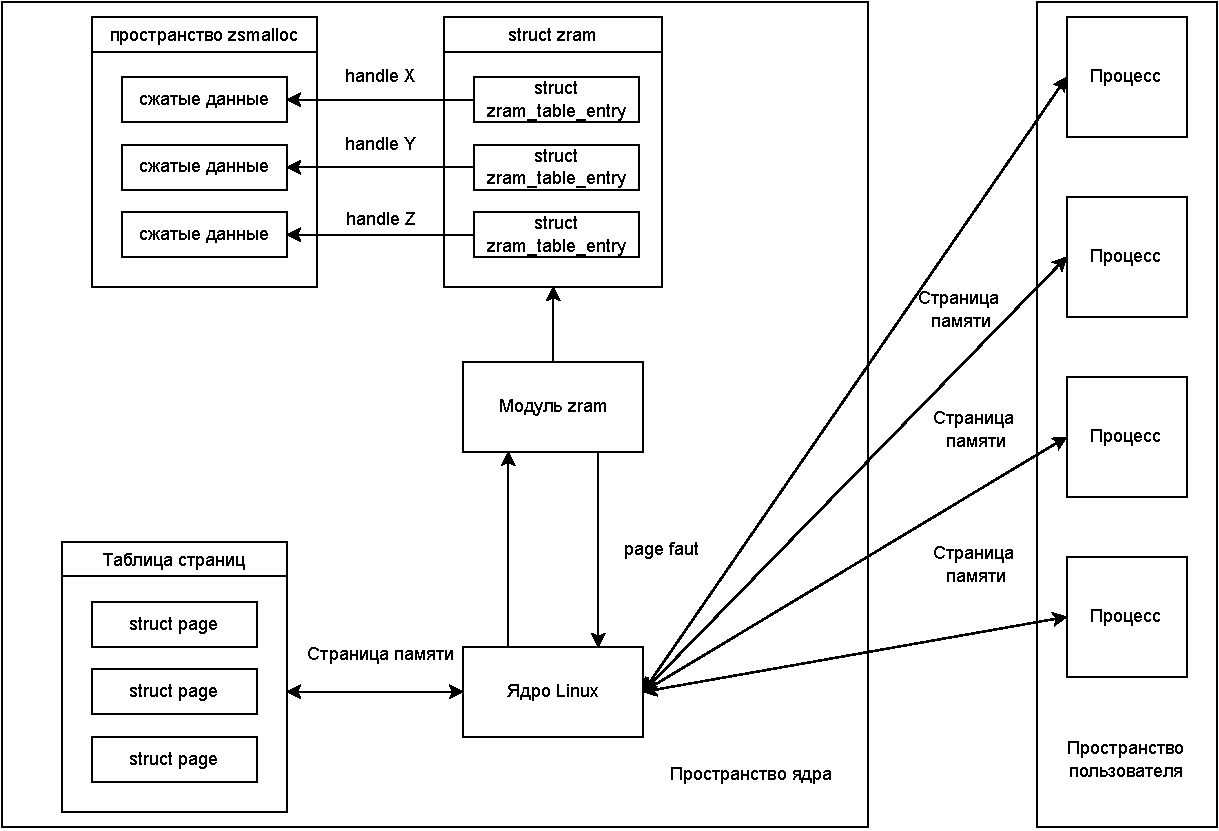
\includegraphics[width=\textwidth]{img/zram-arch.pdf}
	\caption{Схема работы модуля ядра zram}
	\label{fig:zram}
\end{figure}

Приведем алгоритм работы zram при попытки записи в блочное устройство:

\begin{enumerate}
	\item содержимое каждой страницы памяти, попавшее в блочное устройство, сжимается и записывается во временный буффер;
	\item у аллокатора zsmalloc запрашивается участок памяти, с помощью функции \texttt{zs\_malloc}, равный размеру сжатых данных;
	\item происходит сопоставление закодированного указателя \texttt{handle} и выделенной областью памяти с помощью функции \texttt{zs\_map\_object};
	\item сжатые данные копируются из временного буффера, в область памяти выделенную аллокатором. Временный буффер освобождается.
	\item заполняется соответствующая ячейка массива структур \texttt{zram\_table\_entry}. В структуре сохраняется указатель на объект --  \texttt{handle} и в переменную \texttt{flags} устанавливаются флаги, описывающие сжатые данные обрабатываемой страницы. 
\end{enumerate}

Алгоритм чтения из блочного устройства аналогичен алгоритму записи.

\section{Алгоритм объединения содержимого страниц оперативной памяти}

Рассмотрим ситуацию, представленную на рисунке \ref{fig:zram-duplicates}. 

\begin{figure}[h]
	\centering
	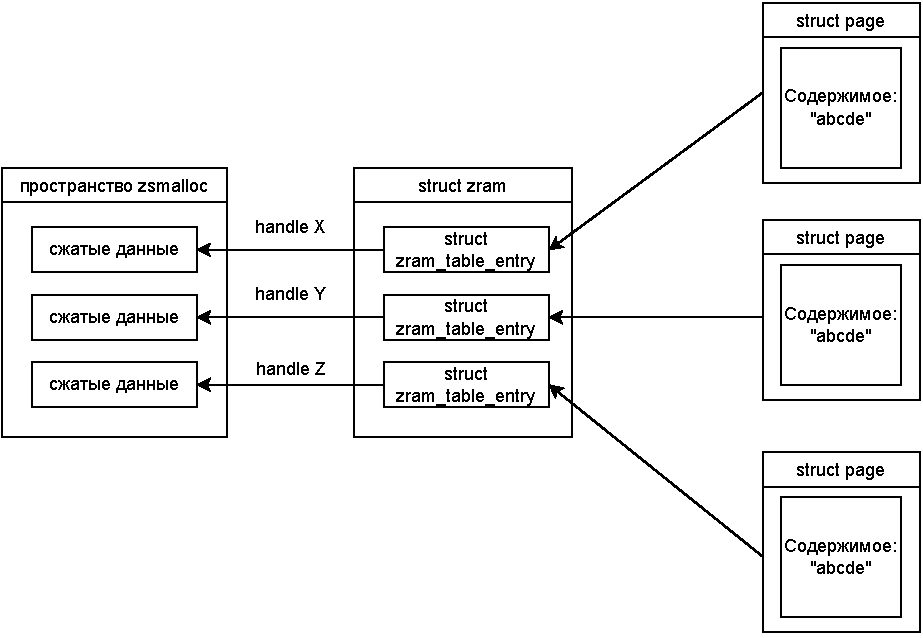
\includegraphics[width=\textwidth]{img/zram-duplicates.pdf}
	\caption{Страницы с одинаковым содержимым}
	\label{fig:zram-duplicates}
\end{figure}

Три страницы с одинаковым содержимым соответствуют трём разным структурам \texttt{struct zram\_table\_entry}, которые в свою очередь хранят закодированный указатель на данные. Сжатые данные, хранящиеся внутри аллокатора zsmalloc, дублируют друг друга. В данном примере, при сжатом размере страницы равным $n$ байт, модуль zram использует $3 * n$ байт памяти, вместо того чтобы использовать $n$ байт. 
Этого можно добиться заменив закодированные указатели \texttt{handle Y} и \texttt{handle Z} на \texttt{handle X}, освободить участки памяти внутри zsmalloc, на которые они указывают и добавить счётчик ссылок на объект, на который указывает \texttt{handle X}. Таким образом, можно сохранить $2 * n$ байт оперативной памяти. Данная оптимизация представлена на рисунке \ref{fig:zram-no-duplicates}.

\begin{figure}[h]
	\centering
	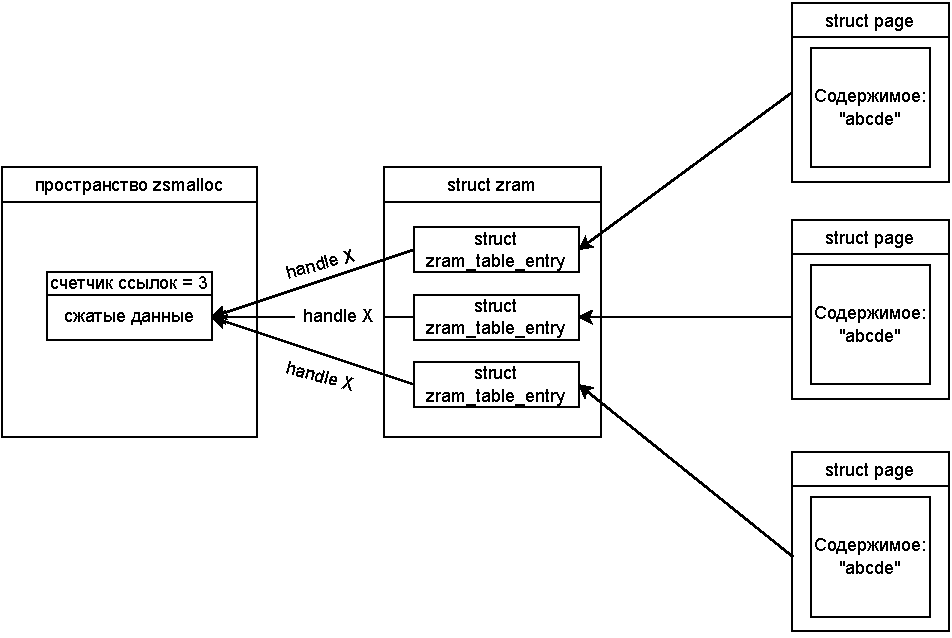
\includegraphics[width=\textwidth]{img/zram-no-duplicates.pdf}
	\caption{Дедупликация данных}
	\label{fig:zram-no-duplicates}
\end{figure}

Алгоритм дедупликации сжатых данных можно описать следующим образом;

\begin{enumerate}
	\item создать хэш-таблицу размерностью $n$, где $n$ -- размер массива структур \texttt{struct zram\_table\_entry};
	\item инициализировать красно-черное дерево, которое будет хранить узлы вида $(key,\ value)$;
	\item начать итерироваться по массиву структур \texttt{struct zram\_table\_entry};
	\item с помощью функции \texttt{zs\_map\_object} получить указатель на область памяти, в которой хранятся сжатые данные, на которые указывает очередной элемент массива с индексом $index$;
	\item скопировать данные во временный буффер и вычислить для них хэш-сумму $h$;
	\item проверить, пуста ли ячейка хэш-таблицы с индексом $i = h \ mod \ n$;
	\item если ячейка пуста, то добавить в неё индекс $index$ и перейти к обработке следующего элемента массива;
	\item в обратном случае, достать из ячейки хэш-таблицы индекс $index_{hash}$ и получить соответствующий элемент массива структур;
	\item повторить шаги г) и д) для этого элемента массива;
	\item сравнить две полученные хэш-суммы;
	\item в случае их несовпадения, перейти к обработке следующего элемента массива;
	\item в обратном случае, с помощью функции \texttt{zs\_free} освободить участок памяти, на который указывает элемент массива с индексом $index$;
	\item заменить указатель $handle$ у элемента массива с индексом $index$ на соответствующий указатель $handle_{hash}$ структуры с индексом $index_{hash}$;
	\item проверить наличие в красно-черном дереве узла с ключом $k = handle_{hash}$;
	\item если узел уже есть в дереве, инкрементировать значение, хранимое в этом узле (счётчик ссылок на объект $handle_{hash}$);
	\item в обратном случае, добавить в дерево узел с ключом $k = handle_{hash}$ и значение $v = 2$ (так как на объект с $handle_{hash}$ на данный момент времени ссылаются два элемента массива);
	\item перейти к обработке следующего элемента массива структур.
\end{enumerate}

Красно-черное дерево необходимо для дальнейшей корректной работы системы. Без него, при попытке освобождения области памяти, выделенной аллокатором, невозможно узнать, ссылается ли кто-либо ещё на эту область памяти. Это может привести к непредсказуемым последствиям для всей системы и ядра в целом. 

При освобождении одного из элемента массива структур \texttt{struct zram\_table\_entry}, например при прочтении страницы из блочного устройства, необходимо проверить наличие в дереве узла с соответствующем ключом, и, в случае если узел найден, декрементировать значение, хранимое в узле (счётчик ссылок на область памяти). Если счётчик равен нулю (или если узел не найден в дереве), необходимо удалить узел из дерева и с помощью функции \texttt{zs\_free} освободить область памяти.

Отличительной чертой красно-черного дерева является быстрый поиск и относительно долгое удаление и добавление узлов (из-за того что дерево каждый раз приходиться балансировать). В силу особенности реализации алгоритма, в дереве чаще будет производиться поиск, чем удаление или добавление, поэтому для реализации алгоритма было выбрано именно красно-черное дерево, а, например, не обычное бинарное дерево поиска.

Алгоритм реализован в виде отдельной функции, которую можно вызвать из пространства пользователя. Таким образом, пользователь сам должен определить подходящий момент для соответствующего вызова. Описанный алгоритм может быть переделан таким образом, чтобы хэш-сумма считалась при первичной обработке страницы -- то есть в тот момент, когда исходная страница только попадает в блочное устройство в несжатом виде. Но, в таком случае, если система работает с разными данными (мало страниц-дубликатов), zram будет тратить процессорное время на вычисление хеш-сумм в пустую, что ухудшит производительность всей системы. Разработанный подход возлагает ответственность за запуск алгоритма на пространство пользователя, с надеждой что алгоритм будет запущен в тот момент, когда внутри блочного устройства уже находится большее количество страниц-дубликатов.

\section{Сравнительный анализ скорости работы разработанного алгоритма}

Очевидно, что алгоритм эффективен (по памяти) только в ситуациях, когда в системе имеются дубликаты. Чем их больше, тем сильнее разработанный алгоритм увеличивает эффективный размер оперативной памяти. Поэтому, сравним скорость работы алгоритма при различных состояниях системы на различных устройствах. Тестирование проводилось на трёх устройствах:

\begin{enumerate}
	\item Система на одном чипе (англ. SoC -- System on Chip) с 4-мя ядрами Cortex-A35:
	
	\begin{itemize}
		\item Имя устройства: Amlogic SOC S905Y4
		\item Процессор: 4 ядра ARM Cortex-A35 @ 2.3 GHz
		\item Память: 4 ГБ DDR4.
	\end{itemize}
	
	\item SoC с 2-мя ядрами Cortex-A35:
	
	\begin{itemize}
		\item Имя устройства: Amlogic SOC A113L
		\item Процессор: 2 ядра ARM Cortex-A35 @ 2.3 GHz
		\item Память: 128 МБ DDR4.
	\end{itemize}
	
	\item Персональный компьютер с 8-ми ядерным процессором AMD Ryzen 7
	
	\begin{itemize}
		\item Имя устройства: персональный компьютер
		\item Процессор: AMD Ryzen 7 3700X 8-Core Processor
		\item Память: 16 ГБ DDR4.
	\end{itemize}
\end{enumerate}

Алгоритм был протестирован в двух состояниях системы:

\begin{itemize}
	\item в системе более 25\% всех данных -- дубликаты;
	\item дубликаты составляют менее 1\% от общего количества данных.
\end{itemize}

В таблице \ref{tbl:results} представлены результаты проведенного тестирования. В ячейках таблицы указано время (в секундах), потраченное на работу алгоритма. Размер исходных данных -- 128 МБ.

\begin{table}[ht]
	\small
	\caption{Результаты тестирования разработанного алгоритма на различных устройствах}
	\label{tbl:results}
	\begin{tabular}{|l|l|l|l|}
		\hline
		Устройство & S905Y4 & A113L & ПК \\ \hline
		25\% дубликатов & 2.4 сек & 2.5 сек & 0.45 сек \\ \hline
		1\% дубликатов & 2.2 сек & 2.34 сек & 0.4 сек \\ \hline
	\end{tabular}
\end{table}

В таблице \ref{tbl:time} представлено время (в секундах), потраченное на сжатие данных, попавших в блочное устройство, созданное модулем ядра zram. Размер исходных данных -- 128 МБ. 

\begin{table}[ht]
	\small
	\caption{Время потраченное на сжатие данных}
	\label{tbl:time}
	\begin{tabular}{|l|l|l|l|}
		\hline
		Устройство & S905Y4 & A113L & ПК \\ \hline
		25\% дубликатов & 23.1 сек & 40.5 сек & 5.2 сек \\ \hline
		1\% дубликатов & 24.1 сек & 39.1 сек & 5.7 сек \\ \hline
	\end{tabular}
\end{table}

По представленным результатам из таблицы \ref{tbl:results} можно сделать вывод о том, что разработанный алгоритм неэффективен когда в системе находится небольшое количество страниц дубликатов -- процессорное время тратится на подсчёт хэш-сумм, но из-за того что дубликатов в системе практически нет, количество доступной (эффективной) оперативной памяти, за счёт объединения страниц, не увеличивается. Это обусловлено тем, что объединение страниц не происходит. В итоге, в замен на потраченное процессорное время система не получает ничего.

В обратном случае, когда в системе находится 25\% страниц-дубликатов, алгоритм отрабатывает практически с такой же скоростью, как и в случае если в системе таких страниц менее 1\%. Но, в этом случае, система получает выигрыш в виде увеличения объема доступной оперативной памяти.

Кроме того, можно отметить, что скорость работы алгоритма сильно зависит от мощности CPU -- чем больше частота процессора, тем быстрее работает алгоритм. При этом, скорость разработанного алгоритма не зависит от количества ядер процессора. Это можно объяснить тем, что алгоритм не является параллельным и выполняется на одном ядре.

Из таблицы \ref{tbl:time} можно сделать вывод, что алгоритм работает быстро, как минимум, относительно времени сжатия данных. Алгоритм дедупликации работает быстрее в 10 - 15 раз, чем само сжатие данных. На основе этого, можно сделать вывод о быстродействии алгоритма.

\section*{Заключение}

Были описаны базовые принципы управления памятью в ядре Linux. Рассмотрены структуры данных модуля ядра zram, описан алгоритм его работы. Разработан алгоритм дедупликации сжатых данных в качестве модификации модуля zram. Проведено тестирование скорости работы алгоритма на различных устройствах. 

Разработанный алгоритм оказался относительно неэффективным на системах с маленьким количеством дублирующихся данных. Наоборот, чем больше в системе повторяющихся данных, тем более эффективен разработанный алгоритм. Так же стоит отметить быстродействие алгоритма -- объединение страниц происходит в среднем в 10 - 15 раз быстрее, чем сам процесс сжатия страниц.

Разработанный алгоритм вместе с результатами его работы были отправлены разработчикам ядра Linux и модуля zram \cite{1}. Результаты работы алгоритма были оценены разработчиками положительно, а сама реализация на данный момент находится на этапе code review, и, возможно, в будущем будет добавлена в основную ветку ядра Linux.

\begin{thebibliography}{5}
	\bibitem{1} zram: introduce merge identical pages mechanism - Alexey Romanov [Электронный ресурс]. -- Режим доступа: https://lore.kernel.org/all/20221121190020.66548-1-avromanov@sberdevices.ru/
\end{thebibliography}

\noindent \textbf{Романов Алексей Васильевич} — студент, МГТУ им. Н. Э. Баумана, кафедра «Программное обеспечение ЭВМ и информационные технологии».


\end{document}
